% !TEX root = CSL 2021.tex

%\subparagraph*{Measuring sensitivity and similarity of programs in a compositional way}
In program semantics one is usually interested in capturing notions of behavioral equivalence between programs. However,  
%\textit{i.e.} to describe when two programs behave in the same way, so that replacing one by the other in any context produces no observable change in the result. However, 
in several fields like approximate \cite{Mittal2016}, incremental \cite{Cai2014, Picallo2019} and probabilistic \cite{10.1109/LICS.2015.64} computation, it is often more useful to be able to describe when two programs behave in a similar, although non equivalent way, so that replacing one by the other in a given context produces a change in the result which can be quantified and bounded in some way.



This idea has motivated much literature on program (pseudo)metrics \cite{ARNOLD1980181, VANBREUGEL20011,Azevedo_de_Amorim_2017, Escardo1999, BAIER1994171,10.1109/LICS.2015.64, 10.1007/978-3-662-44584-6_4, 10.1007/978-3-662-54434-1_13, 10.1145/3209108.3209149}, that is, of semantics in which types are endowed with a notion of distance measuring the differences in their behaviors. This approach has found widespread applications, for example in differential privacy \cite{10.1145/1932681.1863568, 10.1007/978-3-642-29420-4_3, Barthe_2012}, where one is interested in measuring the \emph{sensitivity} of a program, \textit{i.e.} its capacity to amplify changes in its inputs, and in the study of coinductive models of computation \cite{DESHARNAIS2004323, VANBREUGEL2005115, 10.1007/978-3-662-44584-6_4,10.1007/3-540-48224-5_35}.
%
%A similar concern is found in fields like differential privacy \cite{10.1145/1932681.1863568, 10.1007/978-3-642-29420-4_3, Barthe_2012}, where one looks for means to measure the \emph{sensitivity} of a program, that is, of how much a change in the input will affect changes in the output.

 
% More generally, in many situations one wishes to replace some computationally intensive piece of program by a more efficient, although not equivalent, one: t
 
 
% 
%  For example, in the case of the transformation of $\lambda x.\sin(x)$ into $\lambda x.x$, 
% a natural candidate for their ``difference''  would be a function associating a real number $r$, or, say, a closed ball $B$ around $r$, with the \emph{distance} between $\sin(r)$ and $r$ (or with the sup of the distances computed on the points of $B$). 
% 
    
  
%  A  common ground for these approaches is the idea that  of taking program differences as themselves some kind of programs, relating potential errors in input with errors in  output. 

 
  
% 
%  
%% For this reasons, in such frameworks we find two different classes of programs (with different typing structure): \emph{exact} programs, leading from well-defined inputs to well-defined outputs, and \emph{approximate} programs, leading from errors in the input into errors in the output.
%
%
% 
% In this paper we propose a framework to reason about program differences in a contextual way using some kind 
% 
%  
   
 A fundamental aspect to take into account when reasoning about program similarity is that this notion is highly \emph{contextual}. For instance, replacing a program $\lambda x.\sin(x)$ computing the sine function  by the identity function $\lambda x.x$ 
will not product a considerable error if $\lambda x.\sin(x)$
operates in a context in which it is only applied to values close to 0.
%, replacing $f$ will not produce a considerable error. However, this transformation would no longer be justified if $f$ were applied on values far from 0.
Similarly, in numerical methods based on Taylor's polynomials (e.g. Gauss-Newton method), one replaces a 
 computationally intensive piece of program by one which approximates the former only \emph{around some given point}, and in {approximate computing} techniques like \emph{loop perforation} \cite{loopperf} a compiler can be asked to modify the execution of a loop provided this transformation does not exceed some error bound.
 
\subparagraph*{The trade-off between program metrics and higher-order types}



\begin{figure}
\begin{subfigure}{0.48\textwidth}
\parbox[h][3.5cm][c]{\textwidth}{
\adjustbox{center}{$
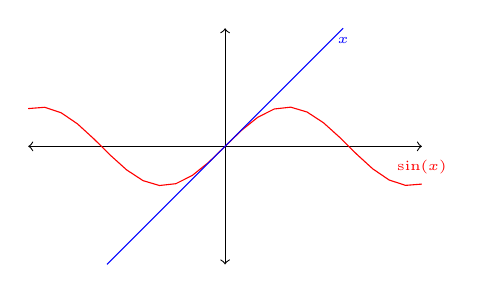
\begin{tikzpicture}[domain=-5:5, scale=0.5]
%\draw[very thin,color=gray] (-0.1,-1.1) grid (3.9,3.9);
\draw[<->]   (-5,0) -- (5,0);
\draw[<->] (0,-3) -- (0,3); % node[above] {$f(x)$};

   % \node at (0,0)[circle,fill,inner sep=1pt]{};
%
\draw[color=red, domain=-5:5] plot (\x, {sin(\x r) } ) node[above] {\tiny$\sin(x)$};

\draw[color=blue, domain=-3:3] plot (\x,{\x  } ) node[below] {\tiny$x$};


\end{tikzpicture}$}
}
\caption{\small $\sin(x)$ and $x$ are very close around 0, but their distance diverges at $\pm \infty$.}
\label{fig:sinid1}
\end{subfigure} \ \ \ 
\begin{subfigure}{0.48\textwidth}
\parbox[h][3.5cm][c]{\textwidth}{
\adjustbox{center}{$
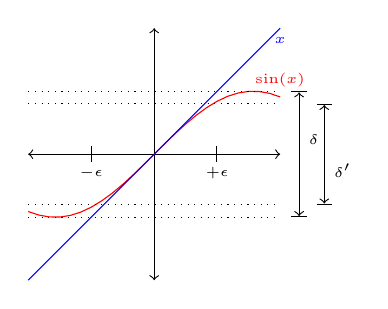
\begin{tikzpicture}[domain=-2:2, scale=0.8]
%\draw[very thin,color=gray] (-0.1,-1.1) grid (3.9,3.9);
\draw[<->]   (-2,0) -- (2,0);
\draw[<->] (0,-2) -- (0,2); % node[above] {$f(x)$};


\draw[|-|] (-1,0) -- (1,0);
\node(r) at (-1,-0.3) {\tiny$-\epsilon$};
\node(r) at (1,-0.3) {\tiny$+\epsilon$};
   % \node at (0,0)[circle,fill,inner sep=1pt]{};
%
\draw[color=red, domain=-2:2] plot (\x, {sin(\x r) } ) node[above] {\tiny$\sin(x)$};

\draw[color=blue, domain=-2:2] plot (\x,{\x  } ) node[below] {\tiny$x$};


\draw[dotted] (-2,1) -- (2,1);
\draw[dotted] (-2,-1) -- (2,-1);

\draw[dotted] (-2,0.8) -- (2,0.8);
\draw[dotted] (-2,-0.8) -- (2,-0.8);

\draw[|<->|] (2.3,1) -- node[above right]{\tiny$\delta$} (2.3,-1);
\draw[|<->|] (2.7,0.8) -- node[below right]{\tiny$\delta'$} (2.7,-0.8);


\end{tikzpicture}$}
}
\caption{\small The self-distances $\delta,\delta'$ of $\sin(x)$ and $x$ in a small interval $[-\epsilon,\epsilon]$ of $0$ are very close.}
\label{fig:sinid}
\end{subfigure} 
\end{figure}
 
 In all cases above one looks for ways to measure the similarity between two programs \emph{in a given context} $\mathtt C[t], \mathtt C[u]$, from a measure of the similarity between $t$ and $u$ and, possibly, of the sensitivity of the context $\mathtt C[\ ]$ itself.  
  While this kind of contextual reasoning is made available in several recent frameworks \cite{10.1145/1932681.1863568,Gaboardi_2013,Azevedo_de_Amorim_2017,chaudhuri, dallago:differential-stlc},  these approaches seem to suggest the existence of a trade-off between the possibility of accounting for 
program differences using program metrics and that of accounting for  a fully higher-order language. Yet, in this paper we propose a framework which accommodates both aspects. 

%
% The question that motivates this paper is whether a notion of program difference of this kind can itself be seen as a metric over the programs of a programming language with higher-order types.  




To be able to formalize the examples discussed above our choice was to start with a language containing a type $\mathsf{Real}$ for real numbers, and to measure errors on this type with the usual metric. Thus, the question we had to answer was how to lift this metric to higher-order types so to enable contextual reasoning.



A standard solution from the literature on program semantics is to define the distance between two programs having a higher-order type $f,g:B\to A$ as the sup of the distances, computed in $A$, between $f(r)$ and $g(r)$, with $r$ ranging on $B$.
This solution works well in models in which programs are interpreted as \emph{non-expansive} or \emph{Lipschitz-continuous} maps between metric spaces \cite{}. However, as is well-known, such models are not \emph{cartesian-closed}\footnote{In fact, cartesian closed categories of metric spaces and non-expansive functions \emph{do} exist \cite{}, but none of these categories contain real numbers with the standard metric.}, hence they do not account for 
 the simply-typed lambda-calculus, but only of linear or sub-exponential variations of it (such as the system $\mathsf{Fuzz}$ \cite{10.1145/1932681.1863568,Gaboardi_2013,Azevedo_de_Amorim_2017}).
 Also, it has been shown \cite{10.1109/LICS.2015.64} that in a probabilistic setting the non-linearity of higher-order programs has the effect of \emph{trivialising} metrics, that is, of forcing distances to be either 0 or 1, hence collapsing program distances onto usual notions of program equivalence.
Moreover, even if one restricts to a sub-exponential language, the sup-distance seems inadequate to account for contextual transformations as the replacement of $\lambda x.\sin(x)$ by $\lambda x.x$,  as the sup-distance between such programs is infinite (see Fig. \ref{fig:sinid1}). 
 
 
On the other side of the coin, the approaches from \cite{chaudhuri, dallago:differential-stlc} are fully contextual and higher-order, but provide, at best, only weak approximations of a standard notion of metric.  
 However, from these approaches we will retain the idea  of taking program differences as being themselves some kind of programs, relating potential errors in input with errors in  output, and thus to separate programs in two different classes (with different typing structure): \emph{exact} programs, leading from well-defined inputs to well-defined outputs, and \emph{approximate} programs, leading from errors in the input into errors in the output.
%

%
%way to lift a metric $d$ on a set $A$ to a set of functions from $B$ to $A$ is by letting the distance between  be defined as the sup of the distances $d(f(x),f(x))$, with $x$ ranging on $B$.
%This approach is at work in several frameworks
%
%
%A standard way to measure differences between programs is by means of program metrics, that is, by endowing types $A$ with a distance $d:A\times A\to \mathbb R^{+}$. However, program metrics usually fail our compositional demand. Typically, in such models the distance between two programs $f,g: \mathsf{Real}\to \mathsf{Real}$ is computed as the $\sup$ of the distances between the values $f(r)$ and $g(r)$, for $r$ a ground element of $\mathsf{Real}$. 
%This approach is then not fine enough to capture differences which might depend on the context. For instance, whenever $g$ is obtained from $f$ by a truncated Taylor expansion around a point $r$, or by the replacement of a  $\mathsf{while}$ loop in $f$ by its perforation, the $\sup$-distance between $f$ and $g$ will most likely be infinite.
%
%
%A second issue with program metrics is that devising models of higher-order programming languages in which types are metric spaces still remains a non-trivial task. In fact, it is well-known that usual categories of metric spaces (\textit{e.g.} those generated by \emph{Lipschitz-continuous} functions)
%%\footnote{An exception is the metric model of PCF in \cite{Escardo1999}, based on a cartesian closed category of \emph{ultrametric spaces}, which in particular excludes $\R$.} \cite{Hofmann2014}) 
%are not \emph{cartesian-closed}, that is, do not provide models of the simply-typed lambda-calculus, but only of linear or sub-exponential variations of it (such as the system $\mathsf{Fuzz}$ \cite{10.1145/1932681.1863568,Gaboardi_2013,Azevedo_de_Amorim_2017}).
%
%
%; 


%second, such models are not at first sight compatible with the compositional approach advocated above: in a metric model the distance between two functional program is a real number (e.g. the max of the distances between the inputs), and this hardly provides a good compositional notion of difference [EXAMPLE HERE, e.g. sin/id, highlight the role of context, you can't justify contextual transformations].

%EXAMPLE: Newton's approximation works well around some point (so it is contextual) -- see Di Cosmo Tweet on Apollo 11






\subparagraph*{Diameter spaces}



In this paper we introduce a class of higher-order denotational models to reason about program similarity and approximate program transformations, that we call \emph{diameter space models}.

In such models a higher-order type $\sigma$ is interpreted by a 4-tuple $A=(|A|, \intervals{A}, \distances{A}, \diam_{A})$, called a \emph{diameter space}, where $|A|$ is a set of \emph{exact} values, $\intervals{A}\subset \mathcal P(|A|)$ is a complete lattice of \emph{approximate} values, $\distances{A}$ is a \emph{quantale}, and $\diam_{A}: \intervals{A}\to \distances{A}$ is a function, called \emph{diameter}, which provides a quantitative measure of approximate values.


In any metric space the distance can be recovered from the diameter function by $d(x,y)=\mathsf{diam}([x,y])$ (where $[x,y]$ is the smallest interval containing $x$ and $y$). Similarly, in a diameter space the function $\diam_{A}$ induces a \emph{generalized partial metric} $d_{A}:|A|\times |A|\to \distances{A}$ by letting $d_{A}(x,y)=\diam_{A}(x\vee y)$ (where $x\vee y$ is the smallest approximate value containing $x$ and $y$). 


Generalized partial metric spaces (henceforth GPMS) are a well-investigated class of metric spaces that has been widely applied in program semantics \cite{}. 
Such spaces generalize standard metric spaces in two ways: they are \emph{generalized} in that distances need not be taken on the standard quantale $\mathbb R^{+\infty}$ of positive reals plus $\infty$, but over an arbitrary quantale, and they are \emph{partial} in that a point can have a self-distance $d(x,x)$ different from 0 (which in turn leads to strengthen the usual triangular inequality as $d(x,y) + d(z,z)\leq d(x,z)+d(z,y)$).\footnote{The adjective ``partial'' comes from the fact that in partial metric semantics like \cite{} the  programs with a non-zero self-distance are those which are not total, in the sense of Scott domains. This will not be the case in our framework. 
}   
Observe that not only any standard metric space is a GPMS, but from from any partial metric $d$ one can retrieve a (generalized) metric $d'$ by letting $d'(x,y)=2d(x,y)-d(x,x)-d(y,y)$.

The appeal to GPMS was somehow forced on us by the necessity, argued above, that the distance between two functional programs like $\lambda x.\sin(x)$ and $\lambda x.x$ must be itself some kind of function. First, this implies that this distance cannot be taken in $\mathbb R^{+\infty}$; instead, in our model $ d_{\mathsf{Real}\to\mathsf{Real}}(\lambda x.\sin(x),\lambda x.x)$ is the function that maps an approximate value on $\mathsf{Real}$ (i.e. a closed interval $a$) onto the sup of the distances between $\sin(x)$ and $ y$, with $x,y$ ranging in $a$. 
This forces then to take $\distances{\mathsf{Real}\to\mathsf{Real}}$ as the quantale of non-decreasing maps from $\intervals{\mathsf{Real}}$ to $\distances{\mathsf{Real}}=\mathbb R^{+\infty}$. 
Second, with this definition, the \emph{self-distance} of $\lambda x.\sin(x)$ (resp. $\lambda x.x$)  is a function that associates each interval $a$ with a value $\leq 2$ (resp. with $\diam(a)$, see Fig: \ref{fig:sinid}), so it is not constantly 0. Moreover, as this example suggests, the self-distances of functional programs behave as sort of derivatives, in particular, $ d_{\mathsf{Real}\to\mathsf{Real}}(f,f)$ is constantly 0 only if $f$ is constant, and moreover self-distances 
 compose through a (lax) chain-rule.


While the closeness of  $\lambda x.\sin(x)$ and $\lambda x.x$ around 0 cannot be expressed in a metric semantics based on the sup-distance, in our framework this will be expressed by the fact that their distance, computed in an interval of 0 with a small enough diameter, is very close to the {self-distances} of both functions (see Fig. \ref{fig:sinid}). 







\subparagraph*{Contributions}
The main two technical contributions of this paper are the following. First, we show that the construction just sketched actually permits to scale the standard  metric for $\mathsf{Real}$ to higher-order types, yielding a partial metric model of a simply typed $\lambda$-calculus with a type of real numbers.
Second, we show that diameter space models can be constructed for potentially any higher-order programming language with a reasonable denotational semantics, by defining, for \emph{any} cartesian closed category $\mathbb C$, a cartesian \emph{lax-}closed category $\mathsf{Diam}(\mathbb C)$, in which exact morphisms coincide with the morphisms of $\mathbb C$. The ``lax'' preservation of cartesian closure reflects the fact that, by composing approximations in a higher-order setting, also their error rates compose (typically, approximating non $\beta$-normal $\lambda$-terms will lead to higher error-rates than approximating their $\beta$-normal forms). 



The generality of our construction shows in particular that our partial metric semantics requires no restrictions (e.g. Lipschitz-continuity) on morphisms, and adapts well to the model one starts with. We consider as examples the category $\mathsf{Diam}(\mathsf{Set} )$, which contains a partial metric on the set \emph{all}  set-theoretic functions from $\mathbb R$ to $\mathbb R$, and the category $\mathsf{Diam}(\mathcal{E}ff)$, where $\mathcal{E}ff$ is the \emph{effective topos}, in which the partial metric [ADD REMARK].


%The step from $\mathbb C$ to $\mathsf{Diam}(\mathbb C)$ preserves the cartesian closed structure in a \emph{lax} way: this reflects the fact that,


%
%
%      
%\subparagraph*{Interval spaces over your favorite higher-order language }
%
%
%%While our framework retains several aspects from existing frameworks for program approximations (\cite{}), it is the first one to provide a clear connection with standard techniques for program metrics. Moreover, 
%Beyond establishing a connection with program metrics, our approach has the advantage of being \emph{language-independent}: To demonstrate this fact we show how to construct, from an arbitrary cartesian closed category $\mathbb C$, an interval space model $\mathcal I(\mathbb C)$ in which exact programs coincide with the arrows in $\mathbb C$. %

%
%which combines both qualitative and quantitative information on $\sigma$. The first two components of $A$ are a set $|A|$ of \emph{exact} programs and a complete lattice $\intervals{A}$ of \emph{approximate} programs.
%
%
%[GPMSs exact/approximate
%The quantitative part can be seen as either a measure on approx. programs or a distance on exact programs
%]
%
%[Generality: categoricity, no restriction on functions]
%
%
%- explain GPMSs
%
%- discuss DMs
%
%- derivative?
%
%
%In such models higher-order types are endowed with the structure of a 
%\emph{generalized partial metric space} (GPMS),
%
%
%
%We recall that a \emph{generalized} metric space is one in which distances need not be measured on the usual quantale of positive reals but over an arbitrary quantale. 
%
%
%The idea of considering program distances as programs themselves forced us to 
%generalize the usual notion of metric space in two directions.
%
% 
%%
%%
%% $|A|$  exact programs in $\sigma$, while $\mathcal I$ is a complete sublattice of $\mathcal P(A)$ whose elements are called \emph{intervals}, and codify approximate programs from $\sigma$. A map of interval spaces similarly comprises both an exact map between points and an approximate (monotone) map between intervals.
%The last two components provide quantitative information on exact and approximate programs:
%$\distances{A}$ is a (commutative and integral) quantale and $\diam_{A}: \intervals{A}\to \distances{A}$ is a function, called \emph{diameter}, which measures the largeness of approximations. 
%
%
%[HERE INTUITION ABOUT DIAMETER]
%
%For the reasons spelled above, whenever we consider intervals over functional programs, the measure of an interval should not be taken in the standard quantale of positive reals. This is why the quantale $\mathbb Q$ may vary across different interval spaces. For example, to measure an interval $a$ of programs from $\mathsf{Real}$ to $\mathsf{Real}$, we will let $\mathbb Q$ be the quantale of monotone maps from real intervals to $\mathbb R^{+\infty}$, and let $\delta(a)$ be the map associating a real interval $b$ with the maximum distance between $f(x),g(y)$, where $x,y\in b$ and $f,g\in a$.  
%
%A fundamental property of the quantitative measure $\delta$ is that it can be equivalently described through a program metric. In fact, by composing $\delta$ with the map associating two exact programs with their least common approximation, one obtains a \emph{partial metric} $d: A\times A \to \mathbb{Q}$ such that the measure $\delta(a)$ of an interval can be computed as the \emph{diameter} of $a$ (that is, as $\sup\{d(x,y)\mid x\in a\}$).
%%
%%by composing $\delta$ with the map $\vee$ associating two exact programs with their least common approximation, we obtain a binary map over exact programs $d= \vee\circ \delta: A\times A\to \mathbb{Q}$, which is in fact a \emph{partial metric}.
%
%
% Partial metrics are a well-investigated class of metrics which is widely applied in program semantics \cite{bkmp:partial-metrics, doi:10.1111/j.1749-6632.1994.tb44144.x, Samet:2013aa}. 
%Such metrics generalize usual metrics by not requiring self-distances to be $0$ (and modifying the triangular law accordingly).
%The appeal to partial metrics was indeed forced on us by compositionality: when $f$ is a functional program, its self-distance $d(f,f)$ must itself be a function relating changes in the input of $f$ with changes in its output, hence a function $f$ such that $d(f,f)$ is constantly $0$ would be one which is not sensitive to its input at all or, in other words, a constant function.   


%[MODIFY WHEN EXAMPLES ARE CLEARER] While being based on a general categorical construction, interval spaces adapt well to the specific features of each language. We show that the approximate programs defined for a specific language L incorporate the features of L, since specific interval structures can be defined starting from programs of L by a pullback operation.
%For instance, if L has a derivative or finite difference operator $\Delta$, then by pulling back over it we can define an interval structure over $\mathsf{Real}\to \mathsf{Real}$ so that the difference between two programs depends, in addition to their behavior, on the behavior of their derivatives.
